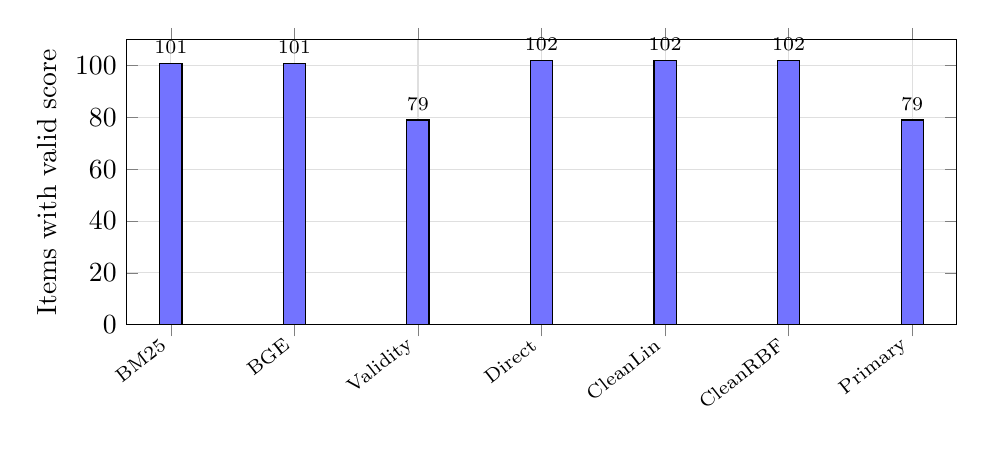
\begin{tikzpicture}
\begin{axis}[
  ybar, bar width=8pt, width=\columnwidth, height=5.2cm,
  ymin=0, ymax=110, ylabel={Items with valid score},
  symbolic x coords={BM25,BGE,Validity,Direct,CleanLin,CleanRBF,Primary},
  xtick=data, x tick label style={rotate=38,anchor=east,font=\scriptsize},
  ytick={0,20,40,60,80,100}, grid=major, major grid style={draw=gray!25},
  nodes near coords, nodes near coords align={vertical},
  every node near coord/.append style={font=\scriptsize},
  enlarge x limits=0.06
]
\addplot[fill=blue!55] coordinates {(BM25,101) (BGE,101) (Validity,79) (Direct,102) (CleanLin,102) (CleanRBF,102) (Primary,79)};
\end{axis}
\end{tikzpicture}
